\documentclass[12pt,english]{article}
\usepackage{geometry}
\geometry{verbose, letterpaper, tmargin = 2.54cm, bmargin = 2.54cm,
  lmargin = 2.54cm, rmargin = 2.54cm}
\geometry{letterpaper}
\usepackage{graphicx}
\usepackage{amsmath}
\usepackage{setspace}
\usepackage{url}
\usepackage{lineno}
\usepackage{xcolor}
\usepackage{bm}
\renewcommand\linenumberfont{\normalfont\tiny\sffamily\color{gray}}
\modulolinenumbers[2]

% Linux Libertine:
\usepackage{textcomp}
\usepackage[sb]{libertine}
\usepackage[varqu,varl]{inconsolata}% sans serif typewriter
\usepackage[libertine,bigdelims,vvarbb]{newtxmath} % bb from STIX
\usepackage[cal=boondoxo]{mathalfa} % mathcal
\useosf % osf for text, not math
\usepackage[supstfm=libertinesups,%
  supscaled=1.2,%
  raised=-.13em]{superiors}

\textheight 22.0cm

\usepackage[round,sectionbib]{natbib}
\bibpunct{(}{)}{;}{a}{}{;}
\bibliographystyle{mee}

\title{Modelling spatiotemporal extremes in ecology}
\author{
Sean C. Anderson$^1$ and
Eric J. Ward$^2$
}
\date{}

\begin{document}

\maketitle

\begin{spacing}{1.25}

  % Point 1: set the context and purpose for the work;
% Point 2: indicate the approach and methods used;
% Point 3: outline the main results;
% Point 4: identify the conclusions, the wider implications and the relevance to management or policy.
% •	Key-words: Provide a maximum of 10 keywords or phrases.

\begin{abstract}

Understanding biological responses to environmental perturbations in time and
space is critical for conservation planning. With projected trends in climate
forcing, for example, conservation biology will have to focus not just on mean
changes, but also on variability and extremes. In ecological systems, extremes
can happen in time, such as population crashes, or in space, such as rapid
range contractions. Here, we introduce a statistical model that extends current
methods for joint inference about temporal and spatial dynamics (spatiotemporal
modelling with Gaussian random fields) to allow for and detect extremes that
occur simultaneously in time and space. Specifically, our model is a Bayesian
predictive-process model that uses a multivariate-t distribution to describe
spatial random effects. The model is easily implemented with our flexible new R
package \textbf{rrfields}, which uses an interface that should be familiar to
anyone who has worked with regression in R. We illustrate applications of our
model and R package simulated and real-world data. First, we \ldots Second, we
predict tree mortality from mountain pine beetle (\emph{Dendroctonus
  ponderosae}) outbreaks in the US Pacific Northwest over the last 16 years. In
both cases, we show that our model provides more accurate and certain
predictions of these ecological processes compared to traditional
spatiotemporal models that do not allow for extremes. Jointly modelling
ecological processes in time and space represents an important step forward to
creating realistic models of anomalies, and allows us to improve predictions
that feed into conservation decisions. Distributing this tool as an R package
should make these models accessible to a wide range of conservation biologists
and scientists in other disciplines interested in predicting extreme events.
\end{abstract}

\section{Introduction}

Applications of statistical models that allow for joint inference about spatial
and temporal dynamics have advanced rapidly in ecology over the last several
decades \citep{bascompte1995, latimer2009}. Spatiotemporal models have also
been widely used in other disciplines, including applications to weather,
remote sensing, human disease dynamics, and crime \citep{cressie2011}. When
ecological data are spatially structured, explicitly accounting for spatial
autocorrelation improves model predictions and inference about parameters of
interest – including recommendations used in management or conservation planning.

Including spatial components in statistical models involves extending models
that most ecologists are already familiar with, such as generalized linear
models (GLMs), generalized additive models (GAMs). Spatial relationships can
be included as predictors in models of the mean (such as in a 2-dimensional
GAM) or can be included in models of the covariance (e.g. kriging). Recent
extensions of these spatial covariance models include modeling spatial
deviations in GLMs or GAMs as multivariate random effects (Gaussian random
fields). Examples of these methods use in existing R packages, include but are
not limited to \textbf{spBayes} \citep{finley2007}, \textbf{spTimer}
\citep{bakar2015}, \textbf{INLA} \citep{rue2009}, \textbf{RandomFields}
\citep{schlather2016}, and \textbf{spate} \citep{sigrist2015}.

A limitation of spatial models that include Gaussian random fields is that
they may perform poorly when underlying data include anomalous or extreme events.
When these models also include an observation model for example, anomalous
observations may be reconciled by increasing the variance of the observation
model (rather than attributing these to extremes in the ecological process being
modeled). Extreme events in temporal processes have been modeled using a variety
of methods in ecology, typically by including finite mixtures of normal and
heavy-tailed distributions \citep{everitt1996, ward2007, thorson2011}. More
recently, the use of the Student-t distribution has been proposed as a robust
solution to modeling process variation in population dynamics (Anderson et al.
in press).

Several robust extensions of Gaussian random fields have been proposed to
better capture extreme spatial events, including applications of max-stable or
extreme value theory \citep{davison2012, davison2012a}. Many of the
applications of these models, such as understanding extremes in rainfall or
flooding, are interested in quantifying the probabilities of exceeding some
threshold \citep{davis2008}. Other extensions of spatiotemporal models to model
extremes include the use of multivariate-t spatial (MVT) random fields
\citep{roislien2007}. Focusing on the latter, to our knowledge these methods
have not been considered for data in the ecology, fisheries, or environmental
sciences.

The objectives of this paper are to introduce the use of robust spatial
predictive models using the multivariate-t distribution, and provide a
user-friendly implementation in our new R package \textbf{rrfields}
(robust random fields). Using simulation testing to compare the multivariate
normal to multivariate-t spatial processes, we illustrate that the multivariate-t
leads to better prediction (less bias, lower uncertainty). We then illustrate
the application of this modeling approach to real-world data that includes
spatial extremes, using data on mountain pine beetle outbreaks in the Pacific
Northwest of the United States. These applications differ in their observation
error model (normal, Gamma) and treatment of temporal change, illustrating the
flexibility of these robust spatial models to other applications in ecology and
related fields.

\section{Methods}

\subsection{Overview}

We seek to allow for large deviations in an ecological spatial pattern over
time by extending a spatiotemporal predictive process model to use a MVT
distribution instead of the usual Gaussian MVN. Below we describe the form of our model
as implemented in \textbf{rrfields}, describe two simulation tests exploring model
performance, and finally describe the application of our model to a data set
representing mountain pine beetle outbreaks in the Pacific Northwest of the
United States.

\subsection{The MVT predictive process model}

\citet{latimer2009} provide an overview of predictive process models for
ecologists. For large datasets that include more than several hundred spatial
locations, estimation of multivariate random effects at the locations of the
data may be computationally prohibitive. One solution to this dimensionality
problem is to estimate the random field as correlated random effects at a
smaller subset of locations or $m$ 'knots' \citep[e.g.][]{latimer2009, shelton2014},
where $m < n$, the number of data points. Instead of estimating an
unconstrained $m \times m$ covariance matrix, a covariance function is
specified \emph{a priori} to estimate the covariance between locations (e.g. exponential,
Gaussian, Matern). Given the estimated random effects at the locations of these knots,
and the known distance matrix between the knots and observed data,
it is straightforward to project or interpolate those random effects to the
locations of observations \citep{latimer2009, finley2009}.

Here, we summarize the important elements of these models and
highlight how our models differs from the usual MVN version. Our model is
essentially a generalized linear model (GLM) with a spatiotemporal element
described by a MVT random field. Our model describes the mean or expected value
of the response, $\mu \equiv \mathbb{E}(y)$, at a set of locations in space $s$
and time $t$ as

\begin{equation}
  g(\mu_{s,t}) = \bm{X}_{s,t} \bm{\beta} + \gamma_{s,t},
\end{equation}

\noindent where $g$ represents a link function (e.g., log, logit, identity),
$\bm{X}_{s,t}$ represents a vector of predictors, and $\bm{\beta}$ represents a
vector of estimated coefficients.
The symbol $\gamma$ represents the spatiotemporal process,
which we describe below.
The variance of the observation component of
our model is a function of the mean via a
probability distribution such as the Gaussian, Poisson, or Gamma.

%A random field is a term used to describe ``random effects'' drawn from a
%multivariate probability distribution representing deviations in a two-dimensional space (REF).
Most commonly, ``random effects'' are represented
as Gaussian random fields using
a MVN distribution with some covariance matrix.
Instead, we draw our values from a (MVT). The MVT
has one extra parameter compared to the MVN: the degrees of freedom parameter
$\nu$. When $\nu$ is small (say $\nu < 10$) the distribution has heavier
tails than the MVN --- it has a higher probability of events far from the mean than the MVN (Fig.~\ref{fig:nu}).
As $\nu$ approaches infinity, the distribution approaches
the MVN. For most purposes, the MVT and MVN are indistinguishable for moderate
values of $\nu$ (say $\nu > 20$) similarly to the univariate t-distribution
compared with the univariate normal distribution \citep[e.g.,][]{anderson2017}.

If $W_{s,t}$ defines a random field, then the spatiotemporal element,
$\gamma_{s,t}$, can be made temporally constant (one field shared across time,
$\gamma_{s,t} = W_{s}$), independent at each time step ($\gamma_{s,t} =
W_{s,t}$), or autoregressive so that the spatial pattern at time $t$ is
dependent on the spatial pattern at time $t-1$ to a degree defined by $\phi$,
($\gamma_{s,t} = \phi \gamma_{s,t-1} + W_{s,t}$).
In the last case,
we constrain the spatiotemporal autoregressive process to be centred on zero at
each time step to aid interpretation and ensure identifiability ($\gamma_{s,t}
= \phi (\gamma_{s,t-1} - \mathbb{E}[\gamma_{t-1}]) + W_{s,t}$). This lets the
mean process be defined by the linear predictor ($\bm{X_{s,t}}\bm{\beta}$)
while $\gamma_{s,t}$ defines the spatial process and how it evolves through
time --- potentially letting ``hotspots'' remain hotspots through time while
keeping the means of the spatial process $\gamma_{s,t}$ stationary and centred
on zero. We determine the location of the $m$ knots in a random field
using the partitioning around
algorithm \citep[the \texttt{pam} function in the R package
\textbf{cluster};][]{reynolds2006}. This algorithm is a robust version of the
common k-means algorithm and results in selecting knot locations that are
proportional to spatial sampling intensity.

We used a squared exponential covariance function to model the covariance
between knot locations. The squared exponential function, $H$,
(also known as the Gaussian covariance function)
is one of the most commonly adopted covariance
functions for spatiotemporal models
and models the correlation between
points $i$ and $j$ as $H(\delta_{ij}) = \exp \left(-\frac{\delta_{ij}^2}{2 \eta} \right)$,
where $\delta_{ij}$ describes the distance between points $i$ and $j$
and $\eta$ describes how steeply correlation declines with increasing distance
or the ``wiggliness'' of the spatial process.
For a given set of $\delta_{ij}$, large values of $\eta$ correspond
to smooth spatial patterns and small values correspondence to wiggly spatial patterns ---
the degree of ``wiggliness'' implied by a value of $\eta$ depends on the scale of the
$\delta_{ij}$.

The elements of the covariance matrix at the $m$ knot locations are therefore
defined as $\Sigma_{ij}^*=\sigma^2 \left( \frac{-\delta_{ij}^2}{2 \eta}  \right)$ with the
parameter $\sigma$ scaling the amplitude of the spatial process deviations. Our
package also allows for the exponential covariance function $H(\delta_{ij}) =
\exp \left(-\frac{\delta_{ij} }{\eta} \right)$ and could be extended to allow for other
common covariance functions such as the Matern or anisotropic covariance
functions in which covariance is not uniform in all directions.
Following \citet{latimer2009}, we can also calculate the covariance matrix
between the locations of the data and the knots,
$\Sigma_{\left(W, W^* \right)}$.
%TODO replace phi
% Each element of the covariance matrix $\Sigma^*$ is thus dependent on
% three quantities: (1) $\delta_{ij}$ the known distance between points $i$ and
% $j$ squared, (2) the scale parameter $\phi$, which determines how steeply the
% correlation declines with increasing distance, and (3) the variance $\sigma^2$.
Given $\Sigma^*$, we can generate random effects at knot
locations by drawing from a MVT distribution for each time step $t$,
$W_t^*\sim \mathrm{MVT}\left( \nu, 0, \Sigma^{*} \right)$.
These random effects at the knots are then projected to the data locations using
$\Sigma_{\left( W,W^{*} \right)}$ \citep{latimer2009}:
$W=\Sigma_{\left(W,W^* \right)}^{'} \Sigma^{*-1}W^*$.

Our package fits these models in a Bayesian framework. We sample
from the posterior distribution using the No-U-Turn Sampler, which is an
extension of Hamiltonian Markov Chain Monte Carlo, implemented in the
statistical software Stan \citep{standevelopmentteam2016a, carpenter2017}
and the R package \textbf{rstan} \citep{standevelopmentteam2016}. Although slower
than an equivalent maximum likelihood approach, this Bayesian approach has a
number of advantages. First, it lets us fully and accurately quantify
uncertainty around all parameter estimates and predictions. This makes it
simple to calculate the probability of specific events happening (e.g., the
probability of abundance falling below some threshold at a given point in space
and time). Given the nature of extreme events, this is likely to be a desired
result from such a model. Second, the Bayesian framework lets us place weakly
informative priors on parameters to impose our existing knowledge of reasonable
values and to aid computation --- particularly of difficult to estimate
parameters such as the degrees of freedom parameter in the MVT. In the case of
the degrees of freedom parameter, $\nu$, we bound the lower value to $2$ for
computational stability and use a Gamma(2, 0.1) prior (i.e., shape = 2, rate = 0.1),
which has a mean of $\sim 20$ and a median of $\sim 17$ \citep{juarez2010}.
If the data are not informative about heavy
tails, our estimate of $\nu$ should approximately match the prior.

%Ju?rez and Steel (2010) (Model-based clustering of non-Gaussian panel data based on skew-t distributions. Journal of Business & Economic Statistics 28, 52?66.)

\subsection{Testing the recovery of extremeness}

We undertook simulation testing to evaluate how well we could recover the degree to
which there were heavy tails in the spatial process under various conditions.
We simulated 50 data points collected at the same survey locations each year
for 5, 15, or 25 years. We simulated the spatial process as independent each
year ($\gamma_{s,t} = W_{s,t}$) with $\sigma^2 = 1$ (the spatial variance),
$\eta = 1$ (the ``wiggliness'' or spatial correlation decay parameter), and
with spatial data locations drawn uniformly from 0 to 10 on both spatial axes
(thereby affecting $\delta_{ij}$, the spatial distances).
We selected 15 knots to represent the spatial pattern as described above.
The simulated degrees of freedom parameter $\nu$ was set at
one of three values: 2.5, 5, or 20, representing very heavy tails, moderately heavy
tails, and effectively normal tails. A final step in our data
simulation was to corrupt the ``true'' data by including measurement or
observation error. We assumed observations to be generated from a gamma
distribution with a log link, $Y_{it}\sim \mathrm{Gamma}\left(a,\frac
  {a}{\mathbb{E}(Y_{it})} \right)$, where the gamma shape parameter $a$ can be
reparameterized into the coefficient of variation (CV), $a=\frac{1}{CV^2}$. We
tested CVs of 0.1, 0.6, and 1.2 representing minimal, moderate, and
considerable measurement error. We set the underlying linear predictor
$\bm{X_{s,t}} \bm{\beta}$ to zero to focus on the spatial process. Therefore,
our simulation model of data $y_{s,t}$ simplifies to

\begin{align}
  \log(\mu_{s,t}) &\sim \mathrm{MVT}\left(\nu, 0, \Sigma_{W(s,t)}\right),\\
  y_{s,t} &\sim \mathrm{Gamma} \left( \frac{1}{\mathrm{CV}^2},
  \frac{1}{\mathrm{CV}^2 \cdot \mu_{s,t} } \right).
\end{align}

We attempted to recapture $\nu$ fitting a model that matched the process
generating the simulated data. We placed weakly informative priors on $\sigma$,
$\eta$, and CV of half-t(3, 0, 3) (i.e., the positive half of a student t
distribution with a degrees of freedom 3, centrality parameter 0, and scale
parameter 3). We initially sampled from each model with 500 iterations across
four chains discarding the first half of the iterations as warm-up. If the
samples had not converged after this initial run, we resampled from the model
with 2000 iterations across four chains. We measured convergence as a minimum
effective sample size of $\ge 100$ and a maximum $\hat{R}$ of $\le 1.05$).

\subsection{Diagnosing the advantage of allowing for extremes}

To evaluate the consequences of assuming a MVN spatial process when the
true spatial process has heavy tails drawn from a MVT, we generated simulated
data sets from a MVT random field and fit models assuming a
MVN random field or the
correct MVT random field.
We then compared the performance of these models. Specifically, we
simulated data from the following model:

\begin{align}
  \mu_{s,t} &\sim \mathrm{MVT}\left(\nu, 0, \Sigma_{W(s,t)}\right),\\
  y_{s,t} &\sim \mathrm{Normal} \left(\mu_{s,t}, \sigma_{\mathrm{obs}} \right),
\end{align}

\noindent with $\sigma^2 = 1$, $\eta = 1$, and 50 spatial data points drawn uniformly
from locations ranging between 0 and 10 along both axes. Again, the locations
of the data, and the 15 knots, were held constant through time to enable faster
computations (this is not a general restriction of the model).
We set the degrees of freedom parameter $\nu$ to 2.5 and used a
Gaussian observation model with standard deviation, $\sigma_{\mathrm{obs}}$, of
0.2. We chose a Gaussian observation
model and identity link for simplicity and to demonstrate an alternative
functional form to the previous simulation. We fit our estimation model as
described above and with a half-t(3,0,3) prior on $\sigma_{\mathrm{obs}}$.

\subsection{Mountain pine beetles in the US Pacific Northwest}

To illustrate real-world applications of MVT-distributed
spatiotemporal models and the \textbf{rrfields} package,
we fit MVT and Gaussian random field models
to a data set representing
mountain pine beetle outbreaks in the
US Pacific Northwest (REF). We modeled the
proportion of grid cells affected by outbreaks
in the US states of XX and XX from 1994 to 2014.
Because the maximum proportion affected was far from 1.0, we
can fit a model with a log link and lognormal observation distribution
(as opposed to a logit link and a beta observation distribution).
The log of the mean proportion affected at location $s$ and time $t$, $\mu_{s,t}$,
is predicted by an initial intercept, $\beta_0$, a year-specific mean estimate, $\beta_t$,
and the spatiotemporal process $\gamma_{s,t}$:

\begin{align}
  \log(\mu_{s,t}) &= \beta_0 + \beta_t + \gamma_{s,t},
  \end{align}

\noindent with the spatial process modeled as autoregressive
and centered at each time step:

\begin{align}
    \gamma_{s,t} &= \phi \left(\gamma_{s,t-1} -
      \mathbb{E}[\gamma_{t-1}]\right) + W_{s,t},\\ \label{eq:beetle-mu}
     W_{s,t} &\sim \mathrm{MVT}\left(\nu, 0, \Sigma_{W(s,t)}\right).
 \end{align}

\noindent Furthermore, we model the annual
mean estimates, $\beta_t$, as following a random walk
constrained by a normal distribution with standard deviation $\sigma_{\beta}$,
and the data, $y_{s,t}$, as generated by a lognormal observation model
with scale parameter $\sigma_{\mathrm{obs}}$:

 \begin{align}
 \beta_t &\sim \mathrm{Normal}\left( \beta_{t-1}, \sigma_{\beta} \right),\\
  y_{s,t} &\sim \mathrm{LogNormal} \left(  \log(\mu_{s,t}), \sigma_{\mathrm{obs}} \right).
 \end{align}

We converted latitude and longitude degrees into UTMs to have a constant
distance relationship throughout the spatial region and divided the UTM values
by $10^5$ to make the range of $\delta_{ij}$ approximately 10 and therefore
place $\eta$ on a reasonable scale.
We rasterized the map into a 500 by 500 grid
and then aggregated this high-resolution grid
into percent cover in a coarser grid reduced by a factor of 25.
This maintained a reasonable resolution
while limiting the data size for rapid model fitting.
We chose 25 knots to represent the spatial process as described above.
We fit the models with half-t(3, 0, 3) priors on all
scale parameters as described above,
a Normal(0, 10) prior on $\beta_0$,
a MVN(0, TODO) prior on $\gamma_{s,t=1}$,
and a Normal(0, 0.5)[-1, 1] prior on $\phi$.

We compared the above MVT
model to a Gaussian random field model in which
$W_{s,t} \sim \mathrm{MVN}\left(\nu, 0, \Sigma_{W(s,t)}\right)$.
To evaluate out-of-sample predictive accuracy we withheld
25 randomly selected data points
per year from the model fitting,
for a total of 400 withheld data points,
or approximately 10\% of the data.
We then evaluated the root mean squared error,
the coverage of credible intervals, and the width of credible intervals
for predictions on these withheld data points
from the MVN and MVT models.
We also compared the leave-one-out information criteria
\citep[LOOIC;][]{vehtari2016}, a Bayesian information criteria that approximates
leave-one-out predictive performance,
between the MVN and MVT models.

% A complete reproducible version of this analysis written in R Markdown is
% available as Supporting Information and at TODO.

\section{Results}

\section{Discussion}

\section{Acknowledgements}

\section{Data Accessibility}
% : To enable readers to locate archived data, authors should list the database and the respective accession numbers or DOIs for all data from the manuscript

All code and data associated with this paper are available at
\url{https://github.com/seananderson/XX} and are archived at
\url{https://zenodo.org/XX}.
The R package \textbf{rrfields} is available at TODO.

\section{Figures}

\begin{figure}[htb]
\begin{center}
  \includegraphics[width=0.7\textwidth]{../figs/pp-illustration.pdf}
\caption{
Illustration of the steps to fitting a predictive process model.
First we observe spatial data, we select knot locations,
and we calculate the covariance between the knots and the observed data.
Then we fit the model with the knots and data remaining constant throughout.
For each MCMC iteration, values are proposed for the
knots, those values are projected from the knots to the locations of the observed data,
and the likelihood is evaluated at the locations of the observed data.}
\label{fig:didactic}
\end{center}
\end{figure}
% Might be good to just clarify the values being proposed are values of observed data - not spatial locations

\clearpage

\begin{figure}[htb]
\begin{center}
  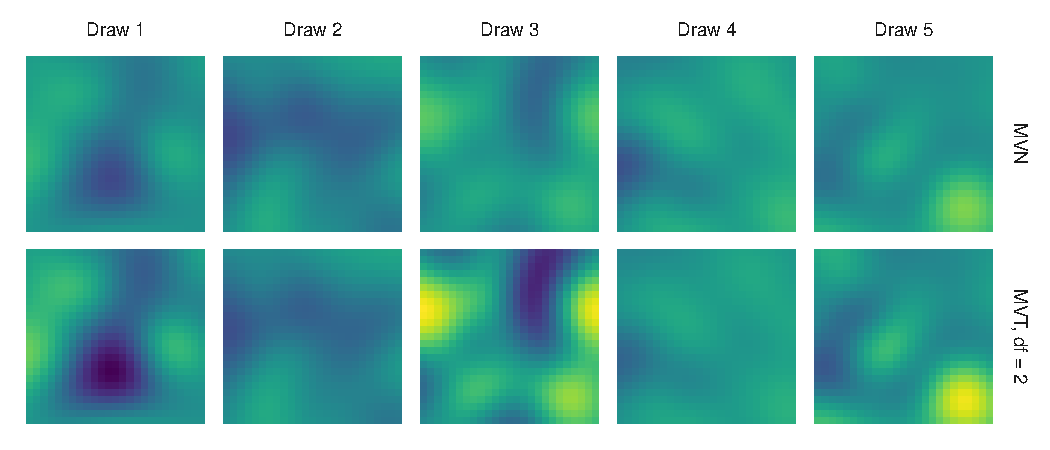
\includegraphics[width=0.9\textwidth]{../figs/nu-rf-illustration.pdf}
\caption{An illustration of five draws from a MVN random field (top row)
vs.\ five draws from a MVT random field with heavy tails
(degrees of freedom, $\nu$, of 2; bottom row). Random seeds are held constant
between the rows
to illustrate the effect. Draws represent slices of time with independent spatial
processes at each time slice. Note the considerably more extreme values in
the third draw for the MVT spatial process.}
\label{fig:nu}
\end{center}
\end{figure}

\clearpage

\begin{figure}[htb]
\begin{center}
  % \includegraphics[width=0.65\textwidth]{../figs/sim-recapture-small.pdf}
  \includegraphics[width=0.85\textwidth]{../figs/recapture-3-base.pdf}
\caption{Results from simulation testing the ability to recapture the degree
of spatial heavy tailedness. Panels show
tests with (a) various true values of $\nu$ (the MVT degrees of freedom parameter),
(b) an increasing number of time steps in the data set (with low observation error),
and (c) an increasing level of observation error (with 25 time steps of data).
The full factorial results are shown in Figure~\ref{fig:recapture-factorial}.
Individual dots show the median estimates from individual simulation runs
with random jitter added on the horizontal axis for visualization.
Polygons show the density of the distribution of estimates.
The colour scale indicates the true degree of heavy tailedness from
yellow (effectively normal) to red (very heavy tailed; $\nu = 2.5$).
The parameter $\nu$ has a lower limit of $2$ in the model
for computational stability.
}
\label{fig:recapture}
\end{center}
\end{figure}

\begin{figure}[htb]
\begin{center}
  \includegraphics[width=0.45\textwidth]{../figs/map.pdf}
\caption{One panel of a multipanel figure.
  Other panels will show posterior and prior densities for $\nu$,
  a photo of mountain pine beetles and pine trees affected by an outbreak,
  and a density plot showing the ratios of credible intervals between the 2 models.
}
\label{fig:map-etc}
\end{center}
\end{figure}

\clearpage

\begin{figure}[htb]
\begin{center}
  \includegraphics[width=0.65\textwidth]{../figs/beetles-mvt-predictions.pdf}
\caption{Predicted severity of mountain pine beetle outbreaks in Washington and
  Oregon State in the United States from 1999 to 2014.
  Shown are medians of the modeled parameter $\mu_{s,t}$ from Equation \ref{eq:beetle-mu}
  --- a spatiotemporal MVT random fields model.
}
\label{fig:beetle-pred}
\end{center}
\end{figure}

\clearpage

\bibliography{spatial-extremes}

\end{spacing}

\section{Supporting Information}

\renewcommand{\thefigure}{S\arabic{figure}}
\renewcommand{\thetable}{S\arabic{table}}
\setcounter{figure}{0}
\setcounter{table}{0}

\begin{figure}[htb]
\begin{center}
  \includegraphics[width=0.90\textwidth]{../figs/sim-recapture.pdf}
\caption{
  Full factorial results from the simulation shown in Fig.~\ref{fig:recapture}.
}
\label{fig:recapture-factorial}
\end{center}
\end{figure}

\end{document}

